
%(BEGIN_QUESTION)
% Copyright 2012, Tony R. Kuphaldt, released under the Creative Commons Attribution License (v 1.0)
% This means you may do almost anything with this work of mine, so long as you give me proper credit

Suppose an NDIR gas analyzer is proposed for measuring the concentration of acetylene (C$_{2}$H$_{2}$) gas in a stream containing a high percentage of hydrocyanic acid (HCN) gas.  The infrared spectra of these two species are shown below:

$$\includegraphics[width=15.5cm]{i01123x01.eps}$$

Identify the gases that should fill each of the cells in this NDIR analyzer:

\vskip 10pt

\begin{itemize}
\item{} Reference cell: \underbar{\hskip 50pt} gas
\vskip 10pt
\item{} Luft detector cells: \underbar{\hskip 50pt} gas
\vskip 10pt
\item{} Filter cells: \underbar{\hskip 50pt} gas {\it or} not necessary at all?
\end{itemize}

\vskip 10pt

If you have reason to believe that the proposed measurement scenario is \underbar{impossible} given these spectra, explain why you think so.

\underbar{file i01123}
%(END_QUESTION)





%(BEGIN_ANSWER)

\begin{itemize}
\item{} Reference cell: \underbar{\bf non-absorbing} gas such as {\bf nitrogen}
\vskip 5pt
\item{} Luft detector cells: \underbar{\bf acetylene} (C$_{2}$H$_{2}$) gas
\vskip 5pt
\item{} Filter cells: \underbar{\bf hydrocyanic acid} (HCN) gas
\end{itemize}

2 points for reference cell gas, 4 points for Luft detector gas, 4 points for filter cell gas.

\vskip 10pt

If a student happens to say that this measurement scenario is impossible, because the two absorption spectra completely overlap, award 8 points.  The two spectra are rather close, but there are some wavelengths of light absorbed by acetylene that are not absorbed by hydrocyanic acid, and therefore measurement is still possible.

%(END_ANSWER)





%(BEGIN_NOTES)

{\bf This question is intended for exams only and not worksheets!}.

%(END_NOTES)


